





React on Metan ylläpitämä avoimeen lähdekoodiin perustuva JavaScript kirjasto,
joka on suunniteltu reaktiivisten käyttöliittymien kehittämiseen\labciteend{react24a}
React suosittelee kehittäjiä rakentamaan sovelluksia uudelleenkäytettävien komponenttien avulla.
Jokainen komponentti sisältää oman rakenteensa, tyylinsä ja käyttäytymisensä, joka tekee niistä helposti siirrettävän ja uudelleenkäytettävän.\labcite{react24a}
Komponenteista voidaan sitten koota monimutkaisia käyttöliittymiä. 
\medskip


Komponentit voidaan kirjoittaa JSX (eng JavaScript XML) syntaksilla, joka mahdollistaa HTML tyylisen kirjoituksen JavaScriptin sekaan.
Tämä tekee React:ista helposti luettavan, ymmärrettävän ja opittavan,
joka on auttanut nostamaan Reactin suosiota yhteen maailman käytetyimmistä käyttöliittymä työkaluista.\labcite{statista23a}
\medskip









\subsubsection{JSX}








JSX on laajennus JavaScriptille, joka antaa kehittäjän kirjoittaa HTML tyylistä syntaksia JavaScriptin sekaan
tehden koodista yksinkertaisempaa ja helpompaa ymmärtää\labciteend{Stephen21}
JSX ei ole ECMAscript standardissa, joten selaimet eivät osaa tulkita sitä,
vaan JSX se on suunniteltu käännettäväksi (eng transpile) johonkin ECMAscript standardia toteuttavalle kielelle.\labcite{Facebook22}
\medskip



Kuvassa \nextImageCount{} luodaan muuttuja helloWorld, jolle annetaan arvoksi HTML "p"{} elementti, jossa teksti on "Hello, World!"{}.
Muuttujien arvot voidaan kirjoittaa HTML tyylisellä JSX syntaksilla, 
joka tekee komponenttien määritelmästä helppoluettavan.
\medskip



\bigskip
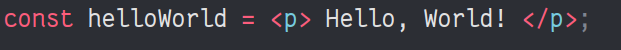
\includegraphics[width=10cm]{src/public/oppar/pure_jsx_example.png}\\
Kuva \getImgCount {}. Esimerki JSX syntaxista
\medskip




Selaimet eivät voi tulkita JSX syntaksia, joten se pitää kääntää natiiviin JavaScriptiin.
Kuvassa \nextImageCount{} on kuvan \theimgCounter{} helloworld muuttuja, joka on käännetty natiiviksi JavaScriptiksi Babel kääntäjää käyttäen.\labcite{babel24}
Tämä antaa selaimille mahdollisuuden suorittaa koodia, joka on alkuperin kirjoitettu JSX syntaksilla.
\medskip


\bigskip
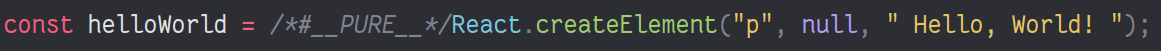
\includegraphics[width=15cm]{src/public/oppar/transpiled_jsx_example.png}\\
Kuva \getImgCount {}. Kuvan \prevImageCount{} JSX-lähdekkoodi käännettynä JavaScriptiin
\medskip





\subsubsection{Komponentit}





Komponentti on oma pieni kokonaisuus, joka sisältää määrittelyt ulkonäölle ja käyttäytymiselle.
Komponentit ovat olennainen rakennusosa React sovelluksissa.
Reactissa Komponentit voivat olla tilallisia tai tilattomia.\labcite{react24b} 
\medskip



Tilaton komponentti ei sisällä omaa tilaa. 
Niiden päätarkoitus on renderöidä käyttöliittymää niille annettujen ominaisuuksien perusteella.
Tilattomat komponentit on helpompi kirjoittaa ja testata. 
Sillä niissä ei saa olla sivuvaikutuksia eikä niiden toiminta tai ulkonäkö muutu sisäisen tilan takia.\labcite{Phuoc23}
\medskip


Tilallinen komponentti tarkoittaa komponenttia, 
joka sisältää oman tilan ja se on vastuussa sen hallinnoinnista ja päivittämisestä.
Tilallisia komponentteja käytetään, kun komponentissa tarvitsee säilyttää dataa ajan myötä 
kuten lomaketietoja.\labcite{Phuoc23}\\
\medskip






React tukee kahta tapaa luoda komponentteja: Luokkakomponentti ja funktiokomponentti.\labciteend{react24c}
Molemmilla komponenttitavoilla voidaan toteuttaa samanlaisia komponentteja, mutta React on suosittelee käyttämään funktiokomponentteja tulevaisuudessa. \labcite{react24c}
Kuvassa \nextImageCount {} on esimerkki tilallisesta funktiokomponentista ja
kuvassa \nextnextImageCount {} on sama laskukomponentti kuin kuva \nextImageCount{} mutta kirjoitettu luokkakomponentti tyylillä. 
\medskip


\bigskip
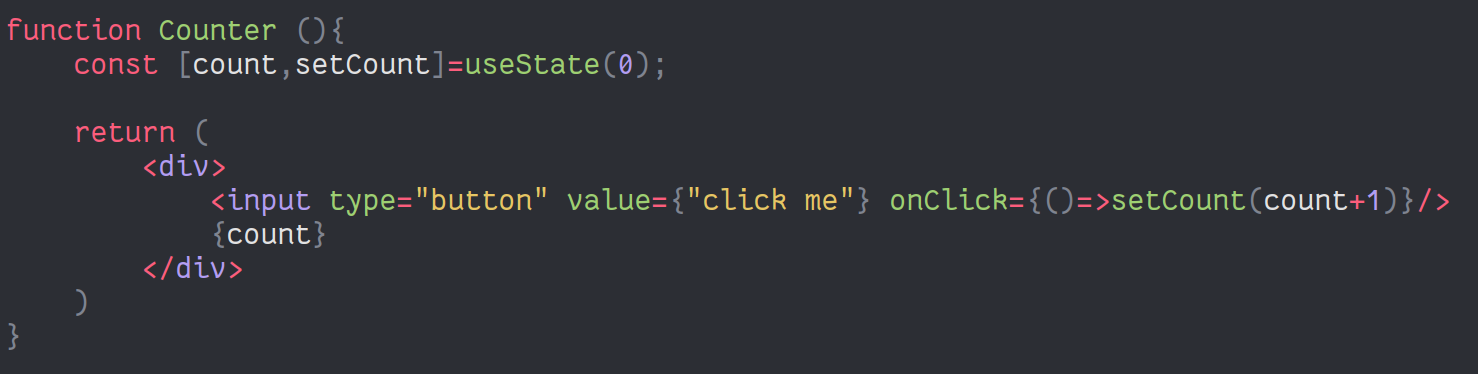
\includegraphics[width=15cm]{src/public/oppar/function_component.png}\\
Kuva \getImgCount{}. React funktiokomponentti
\medskip

Kuvassa \theimgCounter{} määritetään funktiokomponentti, jonka nimeksi on annettu laskija, joka seuraa kuinka monta kertaa nappia on painettu.
Funktio palauttaa komponentin ulkonäön, joka on määritetty JSX syntaksilla.
Komponentissa on myös useState koukku (eng hook), joka tallettaa komponentin tilan.
Tätä käyttäen komponentti pystyy säilyttämään dataa ja päivittämään itsensä, kun sen sisäinen tila muuttuu.
\medskip




\bigskip
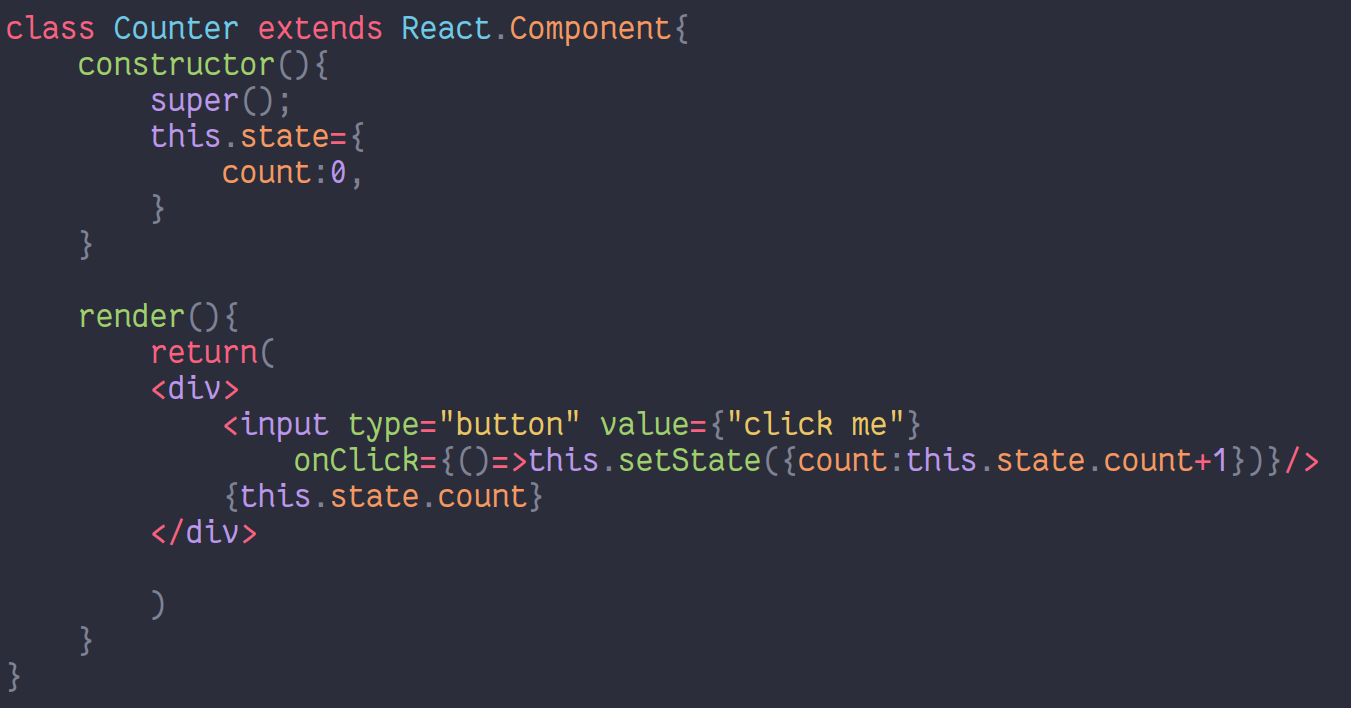
\includegraphics[width=15cm]{src/public/oppar/class_.png}\\
Kuva \getImgCount{}. React luokkakomponentti
\medskip



Luokkakomponentissa komponentin tilaa säilytetään this.state ominaisuudessa, ja sitä voi muuttaa tai päivittää käyttämällä this.setState funktiota. 
Funktio uudelleen renderöi osat komponentista jotka, ovat riippuvaisia kyseisestä tilasta.\labcite{react24c}
\medskip


Funktiokomponentissa tila hallinnoidaan "React hookeilla"{}. 
"Hookit"{} antavat funktiokomponenteille mahdollisuuden käyttää Reactin ominaisuuksia, 
jotka luokkakomponentit saavat, kun ne perivät Reactin "Component"{} luokan.\labcite{react24d}
Kuvan \prevImageCount{} ja \theimgCounter{} komponentit on tehty React 18.3.1 versiolla.
\medskip



\subsubsection{DOM ja VDOM}




DOM (eng Document object model) on rajapinta HTML- ja XML-dokumenteille. 
Se määrittää loogisen rakenteen dokumenteista ja määrittää tavan miten dokumenttia hallinnoidaan.
DOM-mallissa dokumentit esitetään puurakenteella, mutta DOM ei määritä että dokumentit toteutetaan puurakenteella.
Rakenteessa jokainen solmu on objekti, joka esittää osaa dokumentista. 
Soulmuissa voi olla yksi tai useampi objekti ja nämä objektit voivat osoittaa muihin solmuihin.\labcite{w3org}
Kuvassa \nextImageCount{} on esimerkki HTML koodi ja kuvassa \nextnextImageCount {} esimerkki koodi on muotoiltu DOM-puuhun.
\bigskip



    
\begin{tcolorbox}
\begin{lstlisting}[language=html]
<TABLE>
    <ROWS> 
      <TR> 
          <TD>Shady Grove</TD>
          <TD>Aeolian</TD> 
      </TR> 
      <TR>
          <TD>Over the River, Charlie</TD>
          <TD>Dorian</TD> 
      </TR> 
    </ROWS>
</TABLE>
\end{lstlisting}
\end{tcolorbox}
Kuva \getImgCount. Esimerkki HTML-koodi\labimgcite{w3org}
\medskip


Esimerkki HTML koodissa luodaan taulukko, jossa tehdään kaksi riviä ROWS elementin alle. 
Joka riviin tulee sarake, jossa on kaksi "table data"{} elementtiä, jotka sisältävät tekstiä.


\bigskip
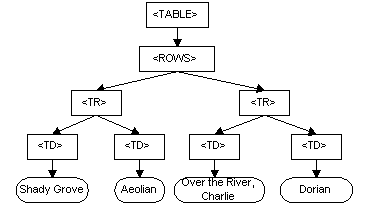
\includegraphics{./src/public/oppar/dom.png}\\
Kuva \getImgCount {}. DOM-puu esimerkki HTML-koodista \labimgcite{w3org}
\medskip



Päivityksien tekeminen DOM-rajapintaa käyttäen on helppoa, mutta hidasta.
Elementin päivittäminen DOM:issa päivittää kyseisen elementin kaikki lapsielementit. 
Tästä päivityksestä voi tulla hyvin hidas, jos elementtejä on paljon.\labcite{refine23}
\bigskip




Käyttöliittymän päivityksien nopeuttamiseksi React on ottanut käyttöön virtuaalisen DOM:in (VDOM).
VDOM on virtuaalinen esitys DOM:ista, jonka React pitää muistissaan koko suorituksen ajan\labciteend{refine23}
Elementtien päivitys yksi kerrallaan DOM:iin jokaisen päivityksen ohessa olisi hidasta,
joten React tekee ensin kaikki päivitykset VDOM:iin, jonka jälkeen DOM:in päivitys voidaan tehdä yhdellä kerralla.
%
%
\medskip

Kun React tekee muutoksia VDOM:iin se luo uuden VDOM-puun, jonka jälkeen
React määrittää mitkä osat käyttöliittymästä ovat muuttuneet vertailu prosessilla (eng diffing).
Vertailu prosessin ansiosta React tietää, mikä on pienin määrä muutoksia, mitä pitää tehdä DOM:iin, 
että käyttöliittymä pysyisi ajan tasalla.\labcite{refine23}
\medskip



